% 安灯常绿队 · 团队补充材料
% 编译器：XeLaTeX（Overleaf: Menu → Compiler → XeLaTeX）
\documentclass[a4paper, 11pt, fontset=fandol]{ctexart}

\usepackage[margin=2.4cm]{geometry}
\usepackage{graphicx}
\usepackage{enumitem}
\usepackage{xcolor}
\usepackage{fancyhdr}
\usepackage[colorlinks=true, linkcolor=black, urlcolor=accent]{hyperref}
\usepackage{xurl}   % 长 URL 任意位置断行，避免溢出行宽

\definecolor{accent}{HTML}{1D4ED8}   % 蓝图蓝，与在线 Demo 视觉一致
\definecolor{soft}{HTML}{555555}

\ctexset{
  section = {format = {\Large\bfseries}, name = {,·}, number = \chinese{section}},
  subsection = {format = {\large\bfseries}},
}

\setlist{itemsep=2pt, topsep=4pt}

\pagestyle{fancy}
\fancyhf{}
\fancyhead[L]{\small\color{soft}安灯常绿队 · 团队补充材料}
\fancyhead[R]{\small\color{soft}\thepage}
\renewcommand{\headrulewidth}{0.3pt}

\linespread{1.25}

\begin{document}

\begin{center}
  {\LARGE\bfseries 团队补充材料}\\[6pt]
  {\large 命题：主动管控设备质量风险的 AI 数字员工（赛力斯 · 生产制造）}\\[8pt]
  {\color{soft}安灯常绿队 · 彭罗健 · 2026-07}
\end{center}

\vspace{4pt}
\noindent
本材料是开题报告的配套补充。一句话：这套方案不是 PPT，是\textbf{在真实工业数据上真的能跑通的系统}——下面每一项都可以点开验证。

\subsection*{核心入口（点开即验）}

\begin{itemize}
  \item \textbf{在线 Demo}（有操作导览、无需装环境）：\url{https://rol1an.github.io/qc-agent-demo/}
  \item \textbf{源码与一键复现}：\url{https://github.com/rol1an/qc-agent-demo}（README 含系统架构图、快速运行、真实运行结果）
  \item \textbf{真实数据分析产物}（仓库内）：\texttt{control\_chart.png}（真实 SPC 控制图，见本文图~\ref{fig:spc}）· \texttt{sample\_run.txt}（完整运行记录）
\end{itemize}

\section{开题报告补充材料}

开题报告正文（Part 1 / Part 2）见报名表。这里补充评委最可能追问的问题与我们的应答。

\subsection*{答辩备题}

\begin{enumerate}
  \item \textbf{「主动」和传统告警的区别？} 传统是越限才报；本方案没报警时也在巡检 SPC 趋势——参数还在规格内、刚出现连续单边或 $C_{pk}$ 下滑，就前瞻立案。是预测，不是事后。
  \item \textbf{「确定性」怎么落地、不是口号？} 一道确定性校验门做三态判定：证据可回溯且不冲突 $\to$ 自动执行低风险处置并复测；不足或矛盾 $\to$ 转人工；本体外实体 $\to$ 拦截。再用 SPC / $C_{pk}$ 把过程能力受控作为质量学意义上的「确定」。
  \item \textbf{会不会乱停线？} 告警先分级、聚合降误报；停线、改参数等高风险动作一律人工确认并留痕。宁可漏报转人工，不乱下发。
  \item \textbf{数据从哪来？} 复用产线既有质检数据（视觉 / CT / 参数）；落地第 0 步先做数据可得性盘点与量具校准（MSA），把「数据可信」作为「结论可信」的前置门。
  \item \textbf{为什么用 Graph RAG？} 一个报警的根因常横跨多道工序，向量检索按相似度召回单点、容易断链；图检索顺着因果链，才能把跨工序的根因串全。
\end{enumerate}

\subsection*{建议 KPI}

均为厂内可自测、与质量强相关：漏检率 DPPM · 误报率（虚警/千次）· 根因命中率 · 处置闭环时延 · 证据链可追溯率 · 过程能力 $C_{pk}$ 回升。

\section{相关项目经验}

\noindent
{\color{soft}\small 注：本材料同时公开于 GitHub。以下按「能力 + 作品」角度陈述、未涉及任何单位。}

\begin{itemize}
  \item \textbf{AI Agent 工程}——大模型 Agent 编排、Graph RAG / 知识库、知识图谱与本体建模、Agent 评测与可靠性工程；擅长把「概率性模型判断」通过规则约束、证据校验、可判定拒答边界，转成「可审计的确定性结论」——正是本方案确定性校验门的方法来源。
  \item \textbf{力学与材料建模}——具备力学、材料失效与有限元 / 仿真背景，对应本方案「故障模式—失效机理」的建模基础。
  \item \textbf{小样本建模}——有在有限数据下做时序 / 分类建模的研究经验，对应「小样本工业数据下给出可靠判断」这一核心难点。
  \item \textbf{本项目}——独立完成本 Demo 全栈：真实数据分析、SPC 引擎、知识图谱、Graph RAG、Agent、三态校验门、可视化前端，已公开可复现。
  \item \textbf{持续学习}——自学 Stanford CS336（从零构建大语言模型），夯实底层原理。
\end{itemize}

\section{数据分析样本}

本方案的数据分析不是示意图，是真实公开工业数据集上的真实计算。

\begin{itemize}
  \item \textbf{数据集}——UCI SECOM（半导体制造过程传感器 $\to$ 合格 / 不合格），1567 批次 × 590 传感器 × 3 个月，公开可下载。
  \item \textbf{样本产物}——图~\ref{fig:spc} 是真实传感器序列上的 SPC 控制图：I-MR 控制限 + 前瞻立案标注 + 滚动 $C_{pk}$；仓库内另有完整运行记录 \texttt{sample\_run.txt}：从真实数据检出 10 个判异事件 $\to$ 三态裁决（自动执行 5 / 转人审 1 / 拦截 1）。
  \item \textbf{分析方法}——数据驱动选过程变量（点二列相关）、I-MR 控制限、Nelson 判异规则、滚动 $C_{pk}$、Graph RAG 跨工序根因检索。
  \item \textbf{换脑对照}——同一数据、同一校验门，只换推理模型：stub 与真 DeepSeek 给出不同根因（膜厚超差 vs 沉积速率漂移），佐证背后是真模型推理、真校验门兜底。
\end{itemize}

\begin{figure}[htbp]
  \centering
  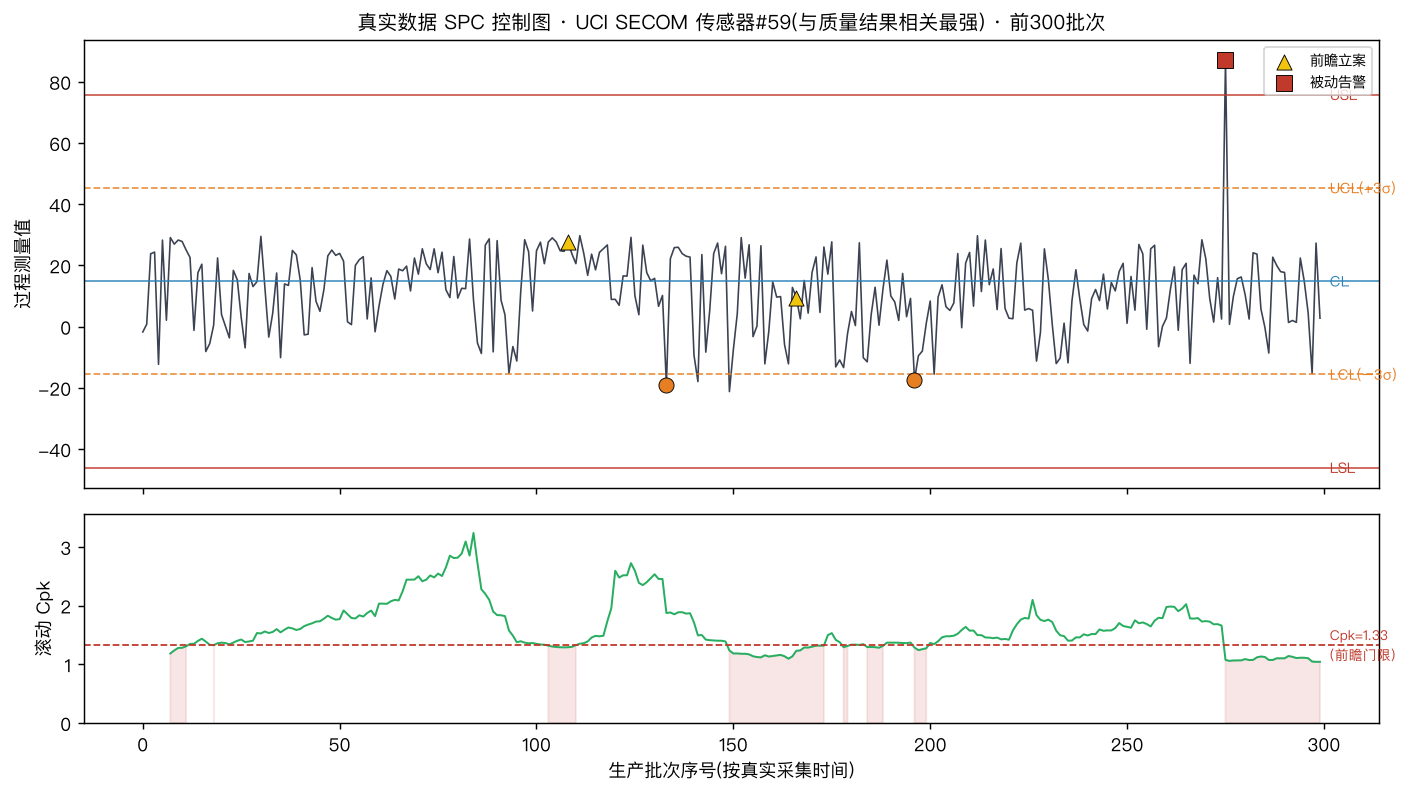
\includegraphics[width=\textwidth]{control_chart.png}
  \caption{真实 SECOM 数据上的 SPC 控制图（I-MR 控制限、判异点标注、滚动 $C_{pk}$），由仓库内 \texttt{src/plot.py} 生成，可一键复现。}
  \label{fig:spc}
\end{figure}

\section{研究笔记（关键决策）}

\begin{itemize}
  \item \textbf{为什么用半导体数据证明汽车命题}——海选拿不到赛力斯真数据；我们不编假汽车数据，而用真实工业数据证明引擎跑得通。引擎与领域解耦——迁移只需换数据接口 + 工艺本体。
  \item \textbf{为什么要「确定性校验门」}——大模型判断是概率性的，工业质量场景不能照单全收。把它收敛成三态确定结果，是本方案与普通问答智能体的根本差异。
  \item \textbf{一个被修掉的漏洞}——三态判定曾有「证据齐全但错」的缺口（知识库过时 / 伪根因自洽会被无兜底执行）；已补上「自动执行后复测确认，未恢复则自动转人审」。
  \item \textbf{主动 vs 被动}——用 SPC 趋势规则（连续单边 / $C_{pk}$ 下滑）在越规格之前介入，即前瞻立案。
\end{itemize}

\section{参考资料清单}

\begin{itemize}
  \item 赛力斯智能制造 · 焊喷 100\% 自动化 / 一车一档：中国质量新闻网 \\ \url{https://www.cqn.com.cn/auto/content/2024-05/30/content_9052218.htm}
  \item 赛力斯整车下线 100\% 全检 / 上万信号：21 经济网 \\ \url{http://www.21jingji.com/article/20241125/herald/f8101344149890a1387c74521b3aedd3.html}
  \item Graph RAG（面向全语料的全局问题检索）：微软 GraphRAG 论文 \\ \url{https://arxiv.org/abs/2404.16130}
  \item 预测性维护 ROI（行业旁证）：Deloitte Insights \\ \url{https://www.deloitte.com/us/en/insights/industry/manufacturing-industrial-products/industry-4-0/using-predictive-technologies-for-asset-maintenance.html}
  \item 数据集 · UCI SECOM：\url{https://archive.ics.uci.edu/ml/machine-learning-databases/secom/}
  \item 方法论：SPC / Nelson 判异规则、FMEA 与控制计划、$C_{pk}$ 过程能力（质量工程通行方法）
\end{itemize}

\vspace{4pt}
\noindent
\textbf{引用纪律}：不写「WEF 全球灯塔工厂」（赛力斯为重庆市级认定）；Deloitte 数字仅作「主动管控值得做」的行业旁证，非本方案对赛力斯的 KPI 承诺；两条赛力斯来源不可互相错挂。

\end{document}
